\documentclass[chicago]{emulateapj}
\usepackage{graphicx,amsmath,natbib,bm}
\usepackage[none]{hyphenat}
\usepackage{amsfonts}
\usepackage[top=1.3in, bottom=-0.3in, left=0.9in, right=0.35in]{geometry}
\usepackage{times}
\linespread{1.01}
\usepackage{enumitem}

\shortauthors{Y. Hezaveh}
\begin{document}

\title{Probing the inner kpc of massive lens galaxies with ALMA: Can the central images of strong lenses be detected?}
\author{Yashar D. Hezaveh, Philip J. Marshall, Roger D. Blandford}  
\affil{Kavli Institute for Particle Astrophysics and Cosmology, Stanford University, Stanford, CA, USA}

\begin{abstract}  
\noindent
We examine the prospects of detecting demagnified images of gravitational lenses in observations of strongly lensed mm-wave molecular emission lines with ALMA. We model the lensing galaxies as a superposition of a dark matter component, a stellar population, and a central supermassive black hole and forecast the detection of the central images for a range of relevant parameters (e.g. stellar core and black hole mass).
We find that over a large range of acceptable parameters, future deep observations of lensed molecular lines with ALMA will be able to detect the central images at $\gtrsim 3\sigma$ significance. We use Fisher analysis to examine the  constraints that could be placed on these parameters in various scenarios. 

\end{abstract}

in Ferarrese 2006, $r_b$ varies from ~50 to 500 pc. 


\keywords{ black hole physics ---
gravitational lensing: strong ---
galaxies: formation ---
galaxies: high-redshift}



\section{introduction}


\begin{figure}
\begin{center}
\centering
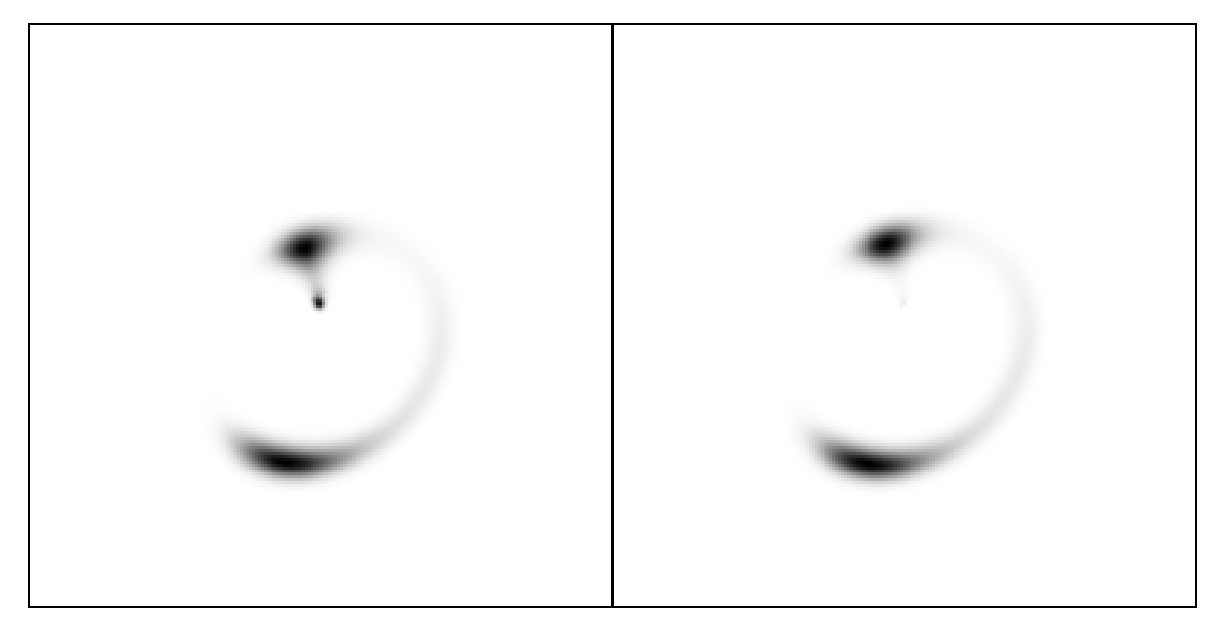
\includegraphics[trim= 0 0 0 0, width=0.48\textwidth]{figures/f_02.eps}
\centering
\end{center}
\caption{ Significance of detection of the central image as a function of the stellar core size. The colors correspond to different slopes of the stellar component. The solid curves correspond to a case without a SMBH while the dashed line show the result of a simulation which includes a $2\times10^8M_{\odot}$ SMBH at its center.
\label{f:f2}}
\end{figure}

\section{Conclusion}

\acknowledgements{
}





\end{document}
